\section{Method}

Notes, this is still a rough draft. 

\subsection{Choice of Research Method}

For this study, I chose to use the experimental design method because it will allow me to isolate the hypothetical impact of the redistricting algorithm from other possible confounding variables. This method also includes the use of a control group, which allows the researcher to establish causation. 

\subsubsection{Components of Experimental Design}

\paragraph{Experimental Units}

The experimental units for this study are the complete datasets for each election year in Viriginia. I have one dataset for each of these years: 2015, 2017, 2019. Every row in each dataset corresponds to a precinct, the smallest geographical unit by which votes are tabulated in Virginia. For each precinct, I have the following attributes: total population, population by race, total voting-age population (VAP)(population over the age of 18), VAP by race, total votes for the democratic House of Delegates (HOD) candidate, total votes for the Republican HOD candidate, and the total votes for any other HOD candidate. Additionally, each precinct has a polygon associated with it that represents its geographical shape. 

\paragraph{Treatments}

The treatments for this study are the three different redistricting algorithm that I'm comparing: Markov chain Monte Carlo \parencite{fifield2020}, Sequential Monte Carlo \parencite{mccartan2020}, and Random Seed Growth \parencite{chen2013}. I'm using the implementations in the R programming language "redist" package \parencite{fifield2020d}. See the Literature Review section for a deeper dive into these algorithms. Broadly, I chose them because they are deterministic. Much of the literature focuses on creating many possible redistricting plans for a commission to choose from, but these three aim to create an "ideal" map. 

\paragraph{Response Variables}

Broadly, the goal will be to evaluate how "fair" each redistricting plan generated by each algorithm for each year is. Within the literature, partisan symmetry is the primary principle used to evaluate redistricting plans. \textcite{katz2020} brings mathematical rigor to the various proposed metrics for measuring partisan symmetry. 

\subparagraph{Partisan Symmetry}

A legislative is said to have partisan symmetry if both parties can receive $m$ proportion of the overall votes and therefore have $n$ proportion of the seats in the legislative body.An example would be that if Republicans win 60\% of the votes but control 65\% of the seats, then in a symmetrical system, Democrats should also be able to control 65\% of the seats by winning 60\% of the votes. \textcite{katz2020}

\begin{figure}
    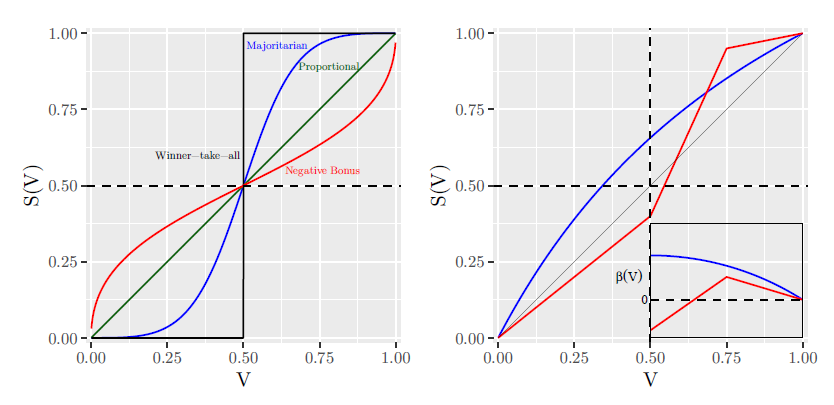
\includegraphics[width=\linewidth]{method/seatsvotes.png}
    \caption{Figure 1: Types of Seats-Votes Curves. Left panel: Symmetric (fair) curves with differing
    levels of electoral responsiveness. Right panel: Asymmetric (biased) curves, including
    one consistently biased toward the Democrats (blue) and one with biases favoring different
    parties depending on V (red); the inset graph is for (V ) for V 2 [0:5; 1] with the vertical
    axis scaled to be the same as the main plot, and lines color coded to the seats-votes curves. \parencite[175]{katz2020}}
    \label{fig:seatsvotes1}
\end{figure}

Partisan symmetry is usually observed by plotting a "seats-votes curve." This plot has $V$, the proportion of the overall votes won by the party, on the x-axis, and $S(V)$, the proportion of the seats won by the party, on the y-axis. Figure \ref{fig:seatsvotes1} \parencite[175]{katz2020} illustrates several hypothetical seats-votes curves.

Naturally, it's very rare to observe the necessary electoral outcomes under the same electoral system in order to determine partisan symmetry. (ie., it's very rare for two parties to tie one year, have one win 51\% of the total votes the next year, and then win 49\% of the votes the following year.)



\subparagraph{Efficiency Gap}

Still need to read about this. 

\subparagraph{Chamber Power Balance}

Since the redistricting that's occuring is hypothetical and I have precinct-level election results for each of these years, I can simulate what the power distribution in the VA House of Delegates would be if the proposed redistricting plan had been used. 

\paragraph{Control Group}

The official VA House of Delegates map used in the years 2015-2019 will serve as the control group for this experiment. I will compute the same metrics for this map as I will for my hypothetical redistricting plans. 

\subsubsection{Principles of Experimental Design}

The primary principles of experimental research design are randomization, replication, and local control. This is how I plan to address them. 

\paragraph{Randomization}

Every experimental unit will receive each treatment, and every experimental unit can be replicated many times without issue, so there’s no error from a lack of randomization. Think of each treatment operating within a separate parallel universe. 

\paragraph{Replication}

There is no need for me to run my trials several times (run the same algorithm on the same data set several times) because these are deterministic algorithms, and the datasets will be immutable. 

\paragraph{Local Control}

All of the redistricting will be happening in controlled environments, so there will be no way for lurking variables to creep in and confound my results. 